%File: q1.tex
%Date: Sun Nov 16 14:03:25 2014 +0800
%Author: Yuxin Wu <ppwwyyxxc@gmail.com>

\section{Introduction}
\begin{frame}
\begin{exampleblock}{\textbf{Project}}
Music understanding and visualization.
\end{exampleblock}

\begin{figure}[H]
  \centering
  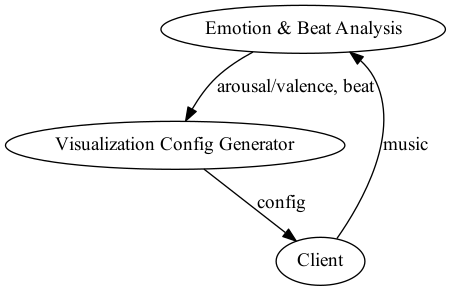
\includegraphics[width=0.7\textwidth]{res/illu.dot.png}
\end{figure}


\end{frame}

\section{Backend Algorithms}
\begin{frame}{Beat Detection}
\begin{enumerate}
    \item Separate percussive and harmonic:
      \begin{enumerate}
        \item Short-time Fourier Transform
        \item Harmonic Percussive Source Separation
        \item Inverse Short-time Fourier Transform
      \end{enumerate}
    \item Detect exact beats from percussive: local estimation with global regularization
  \end{enumerate}
\end{frame}

\begin{frame}{Emotion Detection - Features}
\begin{enumerate}[(a)]
    \item Root Mean Square
    \item High Quefreqncy Log Frequency Spectrum
    \item Chromagram
    \item High Quefrency Chomagram
    \item Mel-frequency Cepstrum
    \item Low Quefrency Log Frequency Spectrum
    \item Log Frequency Spectrum
    \item dbPower
    \item Low Frequency Power
\end{enumerate}
\end{frame}

\begin{frame}{Emotion Detection - Data \& Model}
       \textbf{"Emotion in Music"} public dataset.

     Trained with Gradient Boosting Trees.

     Predict Arousal/Valence of music segments with high accuracy.
\begin{figure}[H]
  \centering
  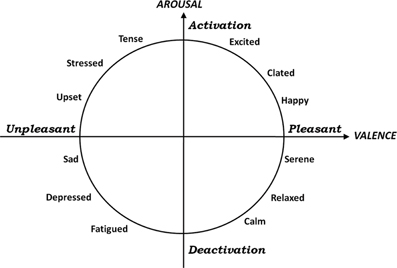
\includegraphics[width=0.6\textwidth]{res/av.jpg}
\end{figure}

\end{frame}

\section{Frontend}
\begin{frame}{3D Tour}
     Use pre-defined visualizations from Light.js/Three.js.

     Show arousal/valence values with HighCharts.js.

     Synchronize with the music using backend analysis results.

Totally differ from old-fashioned music visualization:
\begin{figure}[H]
  \centering
  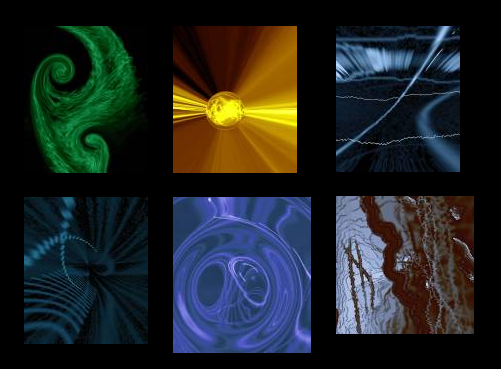
\includegraphics[width=0.6\textwidth]{res/out.png}
\end{figure}

\end{frame}
